\chapter{Network Operations}
	\label{ch:NetworkOperations}
	By using a common language and being able to write it down, the human race has been able to move from hunter gather to large scale society. 
	Language has allowed us to communicate the skills which our forebears learned to their children, eventually to us. 
	In a similar manner, computers need a means of communicating. 
	This is where networking and the OSI model for computer communications comes in, they allow computers to become more than just the machine in front of you. 
	Networking has become commonplace---many people would find no use in a computer without it---and many of our most used programs depend entirely on it. 
	However, to understand how to exploit networking, we need to understand how the communication takes place, how the network has been created and how to connect to the services running on other machines in ways they may not have been designed for. 
	\section{OSI Model}
		When computers are communicating, they need to be able to speak in the same language.\cite{HackingAOE} 
		However, if a programmer needed to implement this every time they required network communication, we would never achieve communication between two systems.\footnote{\url{https://xkcd.com/927/}} 
		Due to this, the OSI Model was created. 
		The OSI model provides the standards for all levels from the application currently being used to the bare metal the data is sent over. 
		These standards allow the relevant equipment to focus on the necessary parts of their implementation, while the other parts are taken care of, allowing for easier communication between unlinked programs. 
		The layers of the OSI Model are as follows:
		\begin{description}
			\item[Physical Layer]
				Deals with the physical connection between two machines through means such as CAT5 Ethernet. 
				This is the lowest layer, whose primary role is communicating raw bits, as well as starting maintaining and ending the transmission. 
			\item[Link Layer]
				Transfers data between the two points connected by the physical layer. 
				This layer provides some high level functions which allow for error correction and flow control. 
				It also provides a means of activating, maintaining and ending the link. 
				This is the layer that a switch would sit on, 
				using the MAC addresses of the connected devices to direct traffic to the correct device. 
			\item[Network Layer]
				Provides a means of transmitting datagrams from one machine on the network to another. 
				This is the layer where network addresses (IP) are translated into a physical machine address. 
				This is the layer that routers work on, allowing them to direct a packet to the correct machine based on IP address. 
				Due to this, you do not have to specify each hop required for a packet to get to a destination. 
			\item[Transport Layer]
				Provides transparent transfer of data by allowing reliable communication and known protocols. 
				This layer means that higher layers need not worry about reliability of connection. 
				This is implemented though means such as TCP and UDP, both of which have different requirements and functions for transport and error checking. 
				This layer works on maintaining the integrity of individual messages. 
			\item[Session Layer]
				Responsible for establishing and maintaining connections between applications. 
				While the transport layer deals with messages, the session layer works on the ongoing connection between the computers. 
				This would usually deal with multiple messages, and numerous packets. 
				Usually this is implemented in a socket by the OS. 
			\item[Presentation Layer]
				Presents the data to the application which is is being communicated to in a format which is understandable to the application. 
				This is the layer which allows for encryption and data compression. 
				This means that the application itself need not be sending encrypted messages to have secure communications. 
				Instead, it could be wrapping its communication socket in a TLS session which would be securing the communications for it. 
			\item[Application Layer] 
				Keeps track of the requirements of the application and allows it to utilize the data which it received. 
				This is where the data is read into the memory of the program and released to it. 
				This allows the program to interpret and act on the data, giving it to the user or changing how it acts based on it. 
		\end{description}
		When data is transmitted through these layers, it is encapsulated in quanta known as packets. 
		Each of these packets contains the meta-data required for each of the layers of the network model. 
		Starting from the application layer, each layer that the packet passes through will add a new header for it's data, which will not be read until the packet passes through that layer on the other end of it's journey. 
		%TODO: Think about using a figure here to show this encapsulation. 
		This layered nature allows us to connect using sockets, handling only the application and presentation layers and allowing the OS to sort the rest for us.

		It is important to note that each layer of the OSI model need not understand the layers around it. 
		Those below will encapsulate the data within their headers and requirements, while those above will simply send their data to the lower layer. 
		Furthermore, each layer communicates only with the corresponding layer on the other machine. 
		Thus, TCP communicates with TCP and applications communicate with applications. 
		Due to this, layers above can be removed from the stack if not required. 
		However, this is a rare situation, occurring only in situations such as ping. 

		Network architecture is the physical layout of the computers connected using the aforementioned OSI model. 
		This is done through means of routers, switches and hubs connecting computers. 
		Each of these components are known as nodes within the network. 
		Nodes are any item along the way that will receive and either terminate or retransmit data. 

	\section{TCP/IP Model}
		Much like the OSI Model, the TCP/IP model was created in order to standardise the way that computers communicate.\cite{ICND1}
		However, this model was created by the DoD, and has become the model that is used in the modern world. 
		It follows a similar idea to the OSI Model, and the same terms are often used to discuss the TCP/IP model, even though they aren't a part of the specification. 
	
		The TCP/IP Model was created through two means, finding other standards to use or creating Request for Comments submissions. 
		The former of these is the way that the Ethernet standard (IEEE 802.3) was added. 
		The latter is what was used to create the protocols and structure of the model. 

		The layers of the TCP/IP Model can be found in Table \ref{tab:TCPIPModel}
		\begin{table}[htb]
			\centering
				\begin{adjustbox}{max width=1\textwidth}
			\begin{tabular}{| l | l |}
				\hline
				\textbf{TCP/IP layers} & \textbf{Focus of Layer}\\ \hline
				Application & Application data to be sent or recieved\\ \hline
				Transport & Transmission assurance and error recovery\\ \hline
				Network & Data delivery along whole path\\ \hline
				Data Link & Individual link delivery\\ \hline
				Physical & Physical make up of the network\\ \hline
			\end{tabular}
		\end{adjustbox}
			\caption{TCP/IP Networking Model}
			\label{tab:TCPIPModel}
		\end{table}

		The Layers of the TCP/IP Model cause one of two types of interaction to occur. 
		\begin{description}
			\item[Same Layer Interaction:] Interaction between machines on the same layer of the TCP/IP Model. 
				This is used to transmit data between machines. 
				Only the layer that sent a particular piece of data will read that data. 
			\item[Adjacent Layer Interaciton:] Interaction between layers on the same machine. 
				This is used to encapsulate data from a higher layer or deliver data from a lower layer. 
				This is used as each layer needs the services of the layer below it in order to send the packet and have it received at the destination. 
		\end{description}

		The TCP/IP Model also specifies the manner in which IP will be used. 
		This allows it to control routing within a network as large as the internet, 
		ensuring that it has a way to get a packet from a source to the destination. 

		This is done using IP routing and subnetting, which lets nodes along the route know approximately where to send a packet. 
		This process leads to the packet eventually being received by a node that is within the same LAN as the destination and forwarding it to it. 

	
	\section{Connecting to Networked Software}
		There are a number of pieces of networked software available. 
		These are often designed to be accessed in a specific manner, however, these can also often be accessed though other tools. 
		Often, you will have one end of a program, usually the server running on another machine. 
		This means that you will have to connect to the in a manner which they were not designed for, 
		reverse engineering the protocol until you have something that works. 

		\subsection{Netcat}
			The first method of doing this is using the tool Netcat or ``ncat''. 
			This tool will connect you to a port, sending any line that you type and printing anything received. 
			This will allow you to connect directly to any networked program with an open port.
			This means that you can determine how the program works, reverse engineering it in order to write your own client for it or access the data it contains. 

			To use this, run the command ``ncat <target> <port>''. 
			This will give you a basic socket connection as previously described to whatever program is working on the given port of the remote machine. 
			You can use ncat for other means, such as creating a shell on another computer. 
			However, this is outside the scope of this section. 
			Further information can be found on the \href{https://nmap.org/book/ncat-man.html}{Ncat Reference Guide}

		\subsection{Programming an Interface}
			This is the means of taking a server application that you have reverse engineered and implementing a client for it. 
			This will give you a usable interface which will automatically interact with the server. 
			Using this will allow you to automate functions such as handshakes and challenge-response sequences. 

			Using the python code learned in Chapter \ref{ch:Programming}, 
			you should be able to write a simple socket script which will respond for you or give you a useful prompt when working with networked software. 

			To test this, set up the \href{https://github.com/CySCA/CySCA2014/blob/master/misc-server/programming/prog01/server.py}{jumbled word server} from \href{https://cyberchallenge.com.au/}{CYSCA 2014} and attempt to write a python script which will run through the challenge response sequence for this server. 

		\subsection{Hidden Services}
			Some services either remain hidden, or refuse to answer until a given task has been completed. 
			The main example of this is port knocking, which forces a user to attempt to connect to a number of ports before the correct one will open. 
			This was created as a means of avoiding port scans, as the ports that are to be used for communications will be closed during the scan. 
			However, it requires either that a process is monitoring the firewall logs, or that the firewall itself is changing based on traffic. 

			This is commonly implemented on ports such as 22 (SSH), which is often a target for brute forcing. 
			The user will set the required ports before enabling the service, opening the SSH port only when the correct sequence has been contacted. 

			Generally, there is no way to determine the sequence required. 
			However, if you are able to read the code being run on the server, you should be able to reverse engineer this sequence and gain access. 

	\section{Domain Name System}
		The Domain Name System (DNS) is the method that is used to translate between domain names such as ``example.org'' to IP addresses such as ``93.184.216.34'' (IPv4) or ``2606:2800:220:1:248:1893:25c8:1946'' (IPv6).
		Without this system, the Internet would be significantly more difficult to navigate, with the dynamic allocation of IP addresses making it impossible to find the same website after reallocation. 
		DNS on the client side makes it possible to access sites by name, removing the need to remember the address and account for its possible changes. 
		However, on the server side, it can be used for numerous activities such as load balancing and regional direction. 

		\subsection{Structure of the Domain Name System}
			DNS is broken down into a number of parts, each of which have authority over a given area. 
			This structure can be thought of as a tree, with each branch delegated responsibility for it's given area. 
			An example of such a tree structure can be found in figure \ref{fig:DNSTree}.

			\begin{figure}[htb]
				\centering
					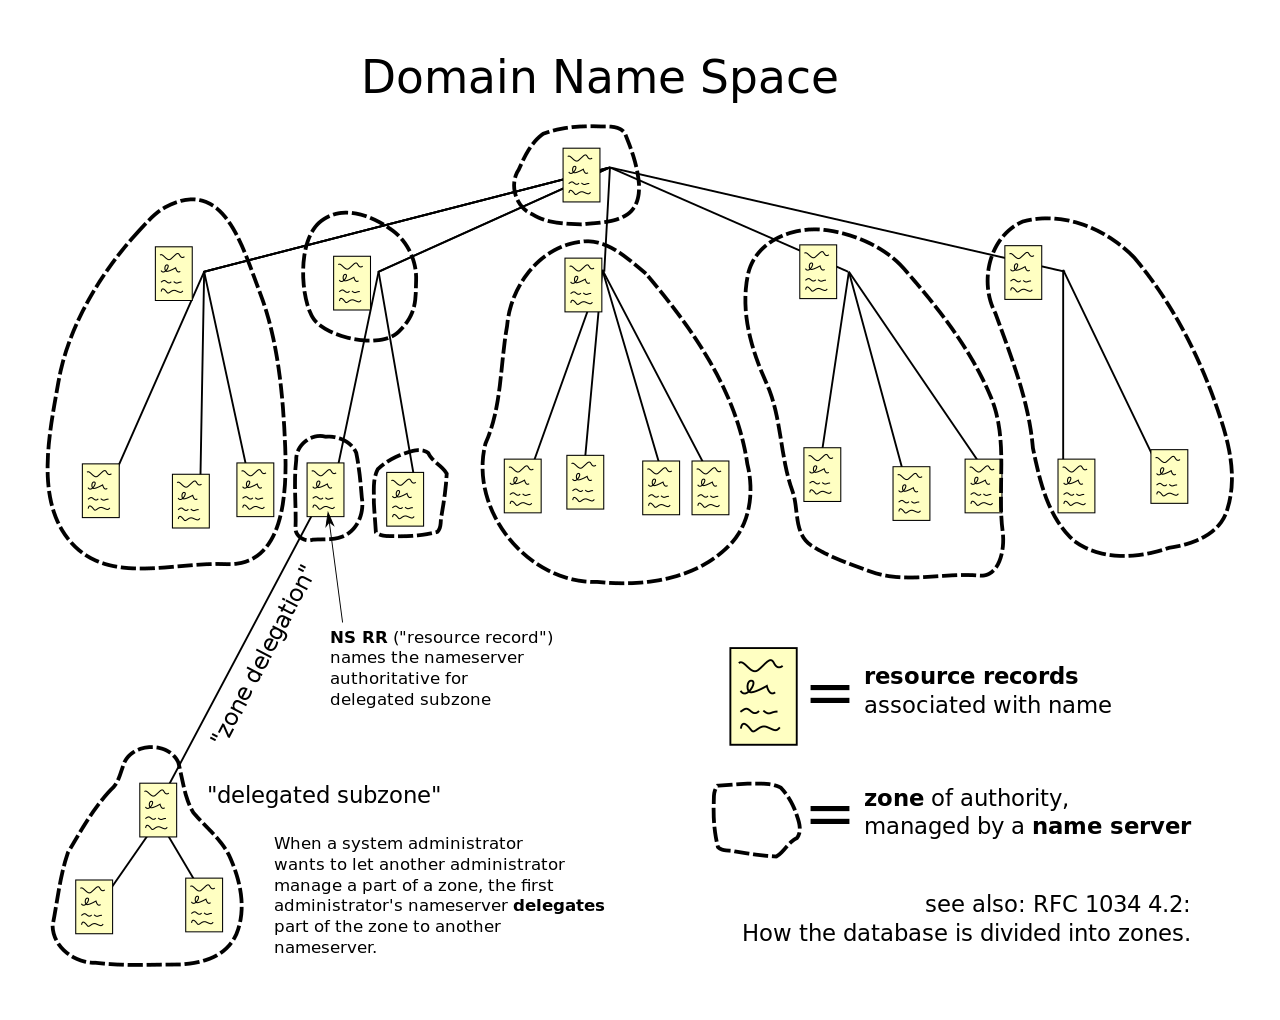
\includegraphics[scale=0.27]{./DNSTree.png}
					\caption{A depiction of DNS for an Internet like network}
					\label{fig:DNSTree}
			\end{figure}

			Within each zone, as indicated by the dashed lines, the top most node is authoritative over the records within that zone. 
			This means that that particular server is the one that is able to reply with the IP address of the name you are looking for, if said name resides within the zone. 
		\subsection{Resolving a Name}
			The process to resolve a name involves a number of steps and a number of servers. 
			Later, we will see that many of these steps can be removed, but it is useful to understand the full system. 
			The servers that will be used are as follows:
			\begin{enumerate}
				\setcounter{enumi}{-1}
				\item Root server (``.'')
				\item TLD server (``.com'')
				\item Authoritative server (``example.com'')
			\end{enumerate}
			The following domain levels will be used in this example:
			\begin{center}
				\begin{tabular}{| c | c | c | c |}
					\hline
					\textbf{Subdomain} & \textbf{Domain} & \textbf{Top Level Domain} & \textbf{Root Domain} \\ \hline
					www & example & com & . \\ \hline
				\end{tabular}
			\end{center}
			The following steps will then be taken to resolve the domain name ``www.example.com'':
			\begin{enumerate}
				\item The Resolver will query a preconfigured root server with ``www.example.com''. 
				\item The Root server will reply with the domain name of the ``.com'' TLD Server.
				\item The Resolver will query the TLD server with ``www.example.com''.
				\item The TLD server will reply with the domain name of the ``example.com'' DNS server. 
				\item The Resolver will query the example.com DNS server with ``www.example.com''. 
				\item The example.com server will reply with the IP address of ``www.example.com'' and that it is the authoritative server for this domain. 
			\end{enumerate}
			It is however, not necessary to go through all of these steps. 
			If we were asking for the address of ``x.y.z.example.com'', the example.com server could respond with the address for this domain if it were configured to be the authoritative DNS server for each of those subdomains. 
			Graphically, such a process would look similar to that shown in figure \ref{fig:DNSRecursor}.

			\begin{figure}[htb]
				\centering
					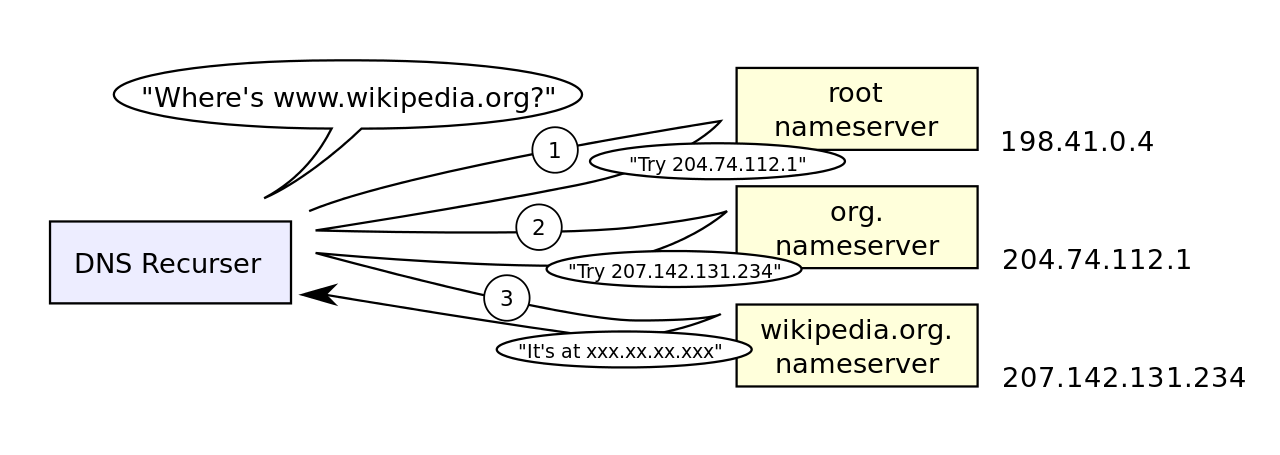
\includegraphics[scale=0.27]{./DNSRecursor.png}
					\caption{A depiction a of recursive DNS lookup}
					\label{fig:DNSRecursor}
			\end{figure}

			Conducting this process for every domain required by the user would result in the root servers and more common TLD servers being overwhelmed by traffic. 
			Furthermore, the resolve times for such a system would be prohibitively long. 
			Due to this, a caching system has been developed to allow many steps of this process to be skipped. 
			This process would likely remove at least the first two steps, but may also remove the third and fourth for more common sites, or sites that the user has accessed recently. 
			Furthermore, a local cache may contain the exact IP address for the site if it has been accessed within the TTL value. 

			When accessing a remote cache, the DNS query may look somewhat like that seen below:
			%TODO: Why is the following not indenting as shown in the source
				\lstinputlisting[numbers=none]{./shellOut/DNSQuery.out}
			The corresponding response may look as follows:
				\lstinputlisting[numbers=none]{./shellOut/DNSResponce.out}
			
			This caching process has been implemented into the DNS structure though the use of Time To Live (TTL) values. 
			This allows the server administrator to set the duration for which a cache can store the address to domain mapping of their server. 
			However, this also means that if their IP address were to change, the TTL would have to be lived out before DNS started pointing at the new IP. 
		\subsection{Protocol Extensions and DNSSEC}
			DNS has been updated to support a number of extensions. 
			These, when unused do not have any overhead on the system. 
			However, when used, they can provide a significant improvement to the system. 
			One such extension is the DNSSEC extension, which provides some security against DNS cache poisoning and other attacks. 

			DNSSEC works through authenticating the packets using digital signing to ensure that the packet came from the server that it was reported to come from. 
			However, this process does not provide any encryption, meaning that DNS packets are readable by anyone sitting between the communicating computers on the network. 

	\section{Hyper Text Transfer Protocol}
		HTTP is a common protocol working on the application layer of the OSI model. 
		This protocol forms the basis for the section of the Internet known as the ``world wide web''. 
		Generally, this protocol would work with the following steps:
		\begin{enumerate}
			\item Client makes request of a server.
			\item Server receives request and returns the requested data along with a status code. 
			\item Client receives and loads data.
		\end{enumerate}

		This simple form can be extended upon by changing what the HTTP server acts upon. 
		For example, a simple PHP site could use the user agent to display a slightly different site to a different browser. 

		HTTP uses the following methods for requesting and sending information:
		\begin{description}
			\item[GET] Requests a resource. These should only retrieve data. 
			\item[HEAD] Identical to the GET method, but without the response body. 
				Useful for meta-information without getting the whole body. 
			\item[POST] Requests that the server accept the data within the request as a subordinate of the URI given. 
				This might be a forum or bulletin board post or data from a web form. 
			\item[PUT] Requests that the data enclosed be stored under the supplied URI. Should modify existing resources. 
			\item[DELETE] Should delete the specified resource. 
			\item[TRACE] Echo back the received request so that the client can determine if intermediaries have altered the request. 
			\item[OPTIONS] Returns the methods that the server supports. 
			\item[CONNECT] Used to connect to HTTPS sites using SSL/TLS through an unencrypted proxy. 
			\item[PATCH] Applies partial modifications to a resource. 
		\end{description}

		Each of these methods has a request and response section, 
		designed to inform either side that the work has completed, as well as sending any required data. 
		Furthermore, to allow interacting programs to understand what has happened on the server, 
		a set of status codes has been created\footnote{\url{http://www.w3.org/Protocols/rfc2616/rfc2616-sec10.html}}. 
		A short list of these is as follows:
		\begin{description}
			\item[2xx] These are the success codes. 
			\item[200] Request has succeeded. Information returned will depend on method used in request. \\
				\textbf{GET:} Corresponding resource sent. \\
				\textbf{HEAD:} The header for the corresponding resource sent. \\
				\textbf{POST:} Entity describing or containing the result of the action. \\
				\textbf{TRACE:} The request message as received by the end server. \\
			\item[201] The request has been fulfilled and resulted in a resource being created. 
			\item[202] The request has been accepted for processing, but has not yet been completed. 
				The client may disconnect, as it will not get another update. 
			\item[3xx] Redirection. 
				This may result in the client taking action to solve the problem for either GET or HEAD requests. 
				Clients should notice and stop infinite redirection. 
			\item[300] There are multiple redirection choices. 
				The user or client should determine which resource should be accessed. 
			\item[301]] Moved permanently. 
				The resource has a new URI, which has been returned in the response body. 
				Client should now move to the new URI. 
			\item[4xx] Client error.
				This is where the clients request does not make sense to the server. 
			\item[400] Bad Request. 
				The request that has been sent contained malformed syntax.
			\item[401] Unauthorised. 
				The current request requires authentication before it can be served. 
			\item[402] Payment Required.
				The request is for a site that is behind a pay wall without the client having paid. 
			\item[403] Forbidden. 
				The server understood but is refusing to fulfill the request. 
				This is lie 401, but authorisation will not change the servers stance. 
			\item[404] Not Found. 
				This status will be returned if the requested URI does not point to a resource. 
			\item[405] Method not allowed. 
				The method used is not allowed for the given URI. 
				The response will include an Allow header containing the valid methods. 
			\item[410] Gone.
				The URI requested has been moved or deleted. 
			\item[5xx] Server Error
			\item[500] Internal server error.
				Server encountered an unexpected condition while processing. 
			\item[501] Server does not support the function requested. 
		\end{description}
	\section{Challenges}
		\subsection{Building a Router}
			This section will take you through the process of building a router on top of a Linux system. 
			This will be a basic router, capable of NAT and packet forwarding, and expandable to contain multiple interfaces and devices such as firewalls. 
			To start this, a number of conventions should be set out:
			\begin{description}
				\item[intern0] The internal pointing network interface. 
					This device points at the LAN. 
				\item[extern0] The external pointing network interface. 
					This device points at the WAN. 
			\end{description}
			When these devices are seen within the configuration of this section, replace them with the equivelent name from your device. 

			\subsubsection{Configuring the Interfaces}
				The interfaces that you will be using for this need to be configured for the setup that you will be using. 
				This can be done through ``netctl'' and the following configuration files:
				File at /etc/netctl/extern0-profile should contain:
				\lstinputlisting[numbers=none]{./shellOut/extern0-profile}
				File at /etc/netctl/intern0-profile should contain:
				\lstinputlisting[numbers=none]{./shellOut/intern0-profile}
				
				
				You will then want to bring these interfaces up using the following commands:
				\begin{lstlisting}[style=CLI]
					$ netctl enable extern0-profile
					$ netctl enable intern0-profile
				\end{lstlisting}

			\subsection{Set up DNS and DHCP}
				You will then want to set up the DNS and DHCP services. 
				The former of these allows your internal machines to communicate with external name servers. 
				The latter allows your router to provide IP addresses to the internal machines. 
				Add the following to the top of ``/etc/dnsmasq.conf'':
				\lstinputlisting[numbers=none]{./shellOut/dnsmasq.conf}
			\subsection{Set up NAT}
				Network Address Translation is the key utility that allows you to communicate through the router. 
				This will allow you to send and receive data through it, and with some configuration, receive incoming connections. 
				In order to set this up, run the following commands in order: 
				\lstinputlisting[style=CLI]{./shellOut/iptablesNat.in}
				I recommend putting these commands into a script file and running that. 
				That way, if you have to make any changes to them or add any new rules, you can put them in the correct place and run the file. 
				Use the command ``iptables -F'' to clear the table before running the script. 

			\subsection{Bring up the services}
				The services that are required will now have to be brought up and enabled for boot. 
				This can be done using the following commands:
				\begin{lstlisting}[style=CLI]
					$ systemctl start dnsmasq
					$ systemctl enable dnsmasq
				\end{lstlisting}
				Furthermore, for information on how the service is running, run the command ``systemctl status dnsmasq''. 

			\subsection{Conclusion} 
				You should now have a fully working router. 
				This can be tested by plugging another machine into the internal interface and attempting to access the WAN. 

				Furthermore, you can continue to configure the router. 
				You may wish to look into firewalls, content filtering, port forwarding, wireless interfaces, packet inspection and SSL offloading in a further attempt to create a secure router and a Cyber Security Operation Center (CSOC) like environment. 
				
